\begin{figure}[H]
\centering
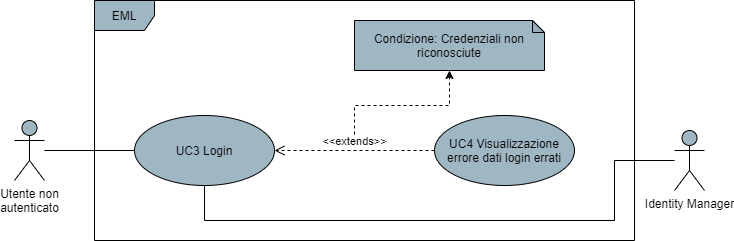
\includegraphics[scale=0.6]{res/UseCase/Immagini/Login}
\caption{Diagramma UML per modulo di login}
\end{figure}

\subsubsection{UCX - Login}
\begin{itemize}
\item \textbf{Attori primari}: utente non autenticato;
\item \textbf{Attori secondari}: identity manager;
\item \textbf{Descrizione}: l'utente, inserendo le proprie credenziali, viene autenticato alla piattaforma;
\item \textbf{Scenario Principale}: l'utente non ancora autenticato richiede l'accesso alla piattaforma dopo aver inserito la propria email e password negli appositi campi dedicati al login;
\item \textbf{Estensioni}:
\begin{itemize}
\item \textbf{UCX}: se le credenziali inserite non vengono riconosciute dall'identity manager, viene visualizzato un messaggio di errore e l'utente viene indirizzato alle pagine di registrazione e di recupero password;
\end{itemize}
\item \textbf{Precondizione}: l'utente prova ad autenticarsi alla piattaforma;
\item \textbf{Postcondizione}: l'utente viene autenticato ed identificato come cliente o venditore/amministratore.
\end{itemize}

\subsubsection{UCX - Visualizzazione errore dati login errati}
\begin{itemize}
\item \textbf{Attori primari}: utente non autenticato;
\item \textbf{Attori secondari}: identity manager;
\item \textbf{Descrizione}: l'utente visualizza un messaggio di errore che lo informa che i dati da lui inseriti durante il login non sono riconosciuti dall'identity manager, indirizzandolo verso le pagine di registrazione e recupero password;
\item \textbf{Scenario Principale}: l'utente tenta di effettuare il login usando credenziali non presenti nel sistema;
\item \textbf{Precondizione}: l'utente prova ad autenticarsi alla piattaforma;
\item \textbf{Postcondizione}: viene visualizzato un messaggio che informa l'utente dell'errore di riconoscimento delle credenziali, e che lo indirizza alle pagine di registrazione e recupero password.
\end{itemize}